\documentclass{standalone}
\usepackage{tikz}
\usetikzlibrary{patterns, positioning}

\begin{document}
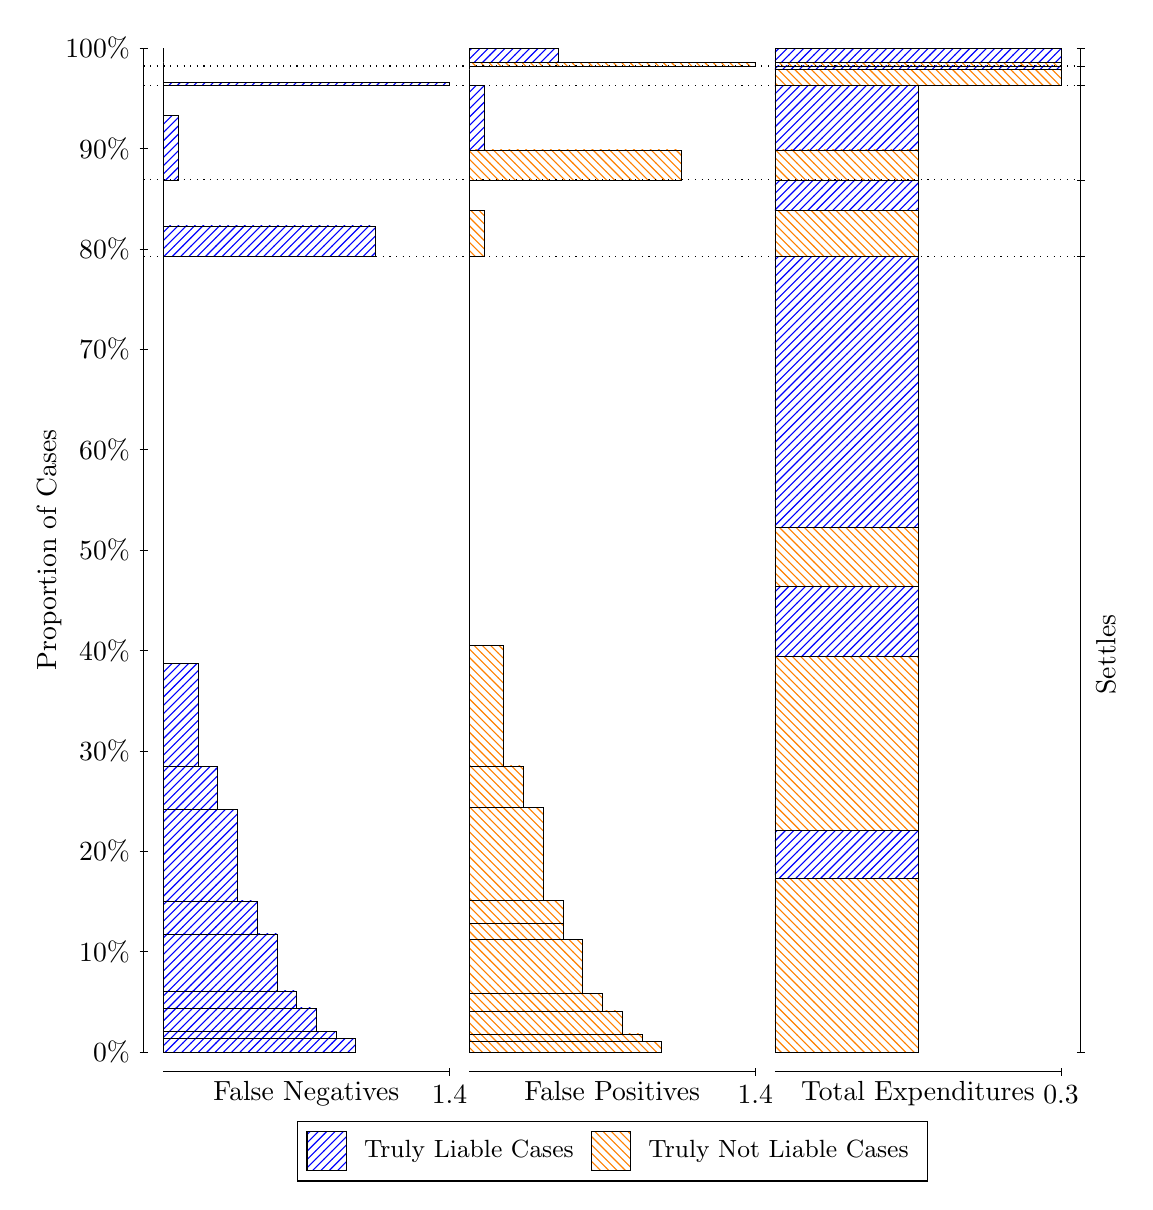
\begin{tikzpicture}
\draw[black, very thin] (1.5,1.75) -- (1.5,14.5);
\node[rotate=90, anchor=center] at (0.3, 8.125) {Proportion of Cases};
\draw[black, very thin] (1.45,1.75) -- (1.55,1.75);
\node[anchor=east] at (1.45, 1.75) {0\%};
\draw[black, very thin] (1.45,3.025) -- (1.55,3.025);
\node[anchor=east] at (1.45, 3.025) {10\%};
\draw[black, very thin] (1.45,4.3) -- (1.55,4.3);
\node[anchor=east] at (1.45, 4.3) {20\%};
\draw[black, very thin] (1.45,5.575) -- (1.55,5.575);
\node[anchor=east] at (1.45, 5.575) {30\%};
\draw[black, very thin] (1.45,6.85) -- (1.55,6.85);
\node[anchor=east] at (1.45, 6.85) {40\%};
\draw[black, very thin] (1.45,8.125) -- (1.55,8.125);
\node[anchor=east] at (1.45, 8.125) {50\%};
\draw[black, very thin] (1.45,9.4) -- (1.55,9.4);
\node[anchor=east] at (1.45, 9.4) {60\%};
\draw[black, very thin] (1.45,10.675) -- (1.55,10.675);
\node[anchor=east] at (1.45, 10.675) {70\%};
\draw[black, very thin] (1.45,11.95) -- (1.55,11.95);
\node[anchor=east] at (1.45, 11.95) {80\%};
\draw[black, very thin] (1.45,13.225) -- (1.55,13.225);
\node[anchor=east] at (1.45, 13.225) {90\%};
\draw[black, very thin] (1.45,14.5) -- (1.55,14.5);
\node[anchor=east] at (1.45, 14.5) {100\%};

\draw[black, very thin] (13.4,1.75) -- (13.4,14.5);
\draw[black, very thin] (13.35,1.75) -- (13.45,1.75);
\node[anchor=west] at (13.35, 1.75) {};
\draw[black, very thin] (13.35,11.849) -- (13.45,11.849);
\node[anchor=west] at (13.35, 11.849) {};
\draw[black, very thin] (13.35,12.826) -- (13.45,12.826);
\node[anchor=west] at (13.35, 12.826) {};
\draw[black, very thin] (13.35,14.022) -- (13.45,14.022);
\node[anchor=west] at (13.35, 14.022) {};
\draw[black, very thin] (13.35,14.272) -- (13.45,14.272);
\node[anchor=west] at (13.35, 14.272) {};
\draw[black, very thin] (13.35,14.5) -- (13.45,14.5);
\node[anchor=west] at (13.35, 14.5) {};

\draw[black, very thin, pattern color=blue, pattern=north east lines] (1.75,1.75) rectangle (4.1931,1.9227);
\draw[black, very thin, pattern color=blue, pattern=north east lines] (1.75,1.9227) rectangle (3.9425,2.0138);
\draw[black, very thin, pattern color=blue, pattern=north east lines] (1.75,2.0138) rectangle (3.692,2.311);
\draw[black, very thin, pattern color=blue, pattern=north east lines] (1.75,2.311) rectangle (3.4414,2.5255);
\draw[black, very thin, pattern color=blue, pattern=north east lines] (1.75,2.5255) rectangle (3.1908,3.2505);
\draw[black, very thin, pattern color=blue, pattern=north east lines] (1.75,3.2505) rectangle (2.9402,3.6693);
\draw[black, very thin, pattern color=blue, pattern=north east lines] (1.75,3.6693) rectangle (2.6897,4.8275);
\draw[black, very thin, pattern color=blue, pattern=north east lines] (1.75,4.8275) rectangle (2.4391,5.3764);
\draw[black, very thin, pattern color=blue, pattern=north east lines] (1.75,5.3764) rectangle (2.1885,6.6881);
\draw[black, very thin, pattern color=orange, pattern=north west lines] (1.75,6.6881) rectangle (1.75,11.849);
\draw[black, very thin, pattern color=blue, pattern=north east lines] (1.75,11.849) rectangle (4.4437,12.241);
\draw[black, very thin, pattern color=orange, pattern=north west lines] (1.75,12.241) rectangle (1.75,12.826);
\draw[black, very thin, pattern color=blue, pattern=north east lines] (1.75,12.826) rectangle (1.9379,13.644);
\draw[black, very thin, pattern color=orange, pattern=north west lines] (1.75,13.644) rectangle (1.75,14.022);
\draw[black, very thin, pattern color=blue, pattern=north east lines] (1.75,14.022) rectangle (5.3833,14.064);
\draw[black, very thin, pattern color=orange, pattern=north west lines] (1.75,14.064) rectangle (1.75,14.272);
\draw[black, very thin, pattern color=orange, pattern=north west lines] (1.75,14.272) rectangle (1.75,14.314);
\draw[black, very thin, pattern color=blue, pattern=north east lines] (1.75,14.314) rectangle (1.75,14.5);
\draw[black, very thin, pattern color=orange, pattern=north west lines] (5.6333,1.75) rectangle (8.0764,1.883);
\draw[black, very thin, pattern color=orange, pattern=north west lines] (5.6333,1.883) rectangle (7.8259,1.9785);
\draw[black, very thin, pattern color=orange, pattern=north west lines] (5.6333,1.9785) rectangle (7.5753,2.2731);
\draw[black, very thin, pattern color=orange, pattern=north west lines] (5.6333,2.2731) rectangle (7.3247,2.4938);
\draw[black, very thin, pattern color=orange, pattern=north west lines] (5.6333,2.4938) rectangle (7.0741,3.176);
\draw[black, very thin, pattern color=orange, pattern=north west lines] (5.6333,3.176) rectangle (6.8236,3.3899);
\draw[black, very thin, pattern color=orange, pattern=north west lines] (5.6333,3.3899) rectangle (6.8236,3.6759);
\draw[black, very thin, pattern color=orange, pattern=north west lines] (5.6333,3.6759) rectangle (6.573,4.855);
\draw[black, very thin, pattern color=orange, pattern=north west lines] (5.6333,4.855) rectangle (6.3224,5.3835);
\draw[black, very thin, pattern color=orange, pattern=north west lines] (5.6333,5.3835) rectangle (6.0718,6.911);
\draw[black, very thin, pattern color=blue, pattern=north east lines] (5.6333,6.911) rectangle (5.6333,11.849);
\draw[black, very thin, pattern color=orange, pattern=north west lines] (5.6333,11.849) rectangle (5.8213,12.435);
\draw[black, very thin, pattern color=blue, pattern=north east lines] (5.6333,12.435) rectangle (5.6333,12.826);
\draw[black, very thin, pattern color=orange, pattern=north west lines] (5.6333,12.826) rectangle (8.327,13.205);
\draw[black, very thin, pattern color=blue, pattern=north east lines] (5.6333,13.205) rectangle (5.8213,14.022);
\draw[black, very thin, pattern color=orange, pattern=north west lines] (5.6333,14.022) rectangle (5.6333,14.23);
\draw[black, very thin, pattern color=blue, pattern=north east lines] (5.6333,14.23) rectangle (5.6333,14.272);
\draw[black, very thin, pattern color=orange, pattern=north west lines] (5.6333,14.272) rectangle (9.2667,14.314);
\draw[black, very thin, pattern color=blue, pattern=north east lines] (5.6333,14.314) rectangle (6.7609,14.5);
\draw[black, very thin, pattern color=orange, pattern=north west lines] (9.5167,1.75) rectangle (11.333,3.9575);
\draw[black, very thin, pattern color=blue, pattern=north east lines] (9.5167,3.9575) rectangle (11.333,4.5603);
\draw[black, very thin, pattern color=orange, pattern=north west lines] (9.5167,4.5603) rectangle (11.333,6.7699);
\draw[black, very thin, pattern color=blue, pattern=north east lines] (9.5167,6.7699) rectangle (11.333,7.6677);
\draw[black, very thin, pattern color=orange, pattern=north west lines] (9.5167,7.6677) rectangle (11.333,8.4115);
\draw[black, very thin, pattern color=blue, pattern=north east lines] (9.5167,8.4115) rectangle (11.333,11.849);
\draw[black, very thin, pattern color=orange, pattern=north west lines] (9.5167,11.849) rectangle (11.333,12.435);
\draw[black, very thin, pattern color=blue, pattern=north east lines] (9.5167,12.435) rectangle (11.333,12.826);
\draw[black, very thin, pattern color=orange, pattern=north west lines] (9.5167,12.826) rectangle (11.333,13.205);
\draw[black, very thin, pattern color=blue, pattern=north east lines] (9.5167,13.205) rectangle (11.333,14.022);
\draw[black, very thin, pattern color=orange, pattern=north west lines] (9.5167,14.022) rectangle (13.15,14.23);
\draw[black, very thin, pattern color=blue, pattern=north east lines] (9.5167,14.23) rectangle (13.15,14.272);
\draw[black, very thin, pattern color=orange, pattern=north west lines] (9.5167,14.272) rectangle (13.15,14.314);
\draw[black, very thin, pattern color=blue, pattern=north east lines] (9.5167,14.314) rectangle (13.15,14.5);
\draw[black, dotted] (1.5,11.849) -- (13.4,11.849);
\draw[black, dotted] (1.5,12.826) -- (13.4,12.826);
\draw[black, dotted] (1.5,14.022) -- (13.4,14.022);
\draw[black, dotted] (1.5,14.272) -- (13.4,14.272);
\draw[black, very thin] (1.75,1.5) -- (5.3833,1.5);
\node[anchor=north] at (3.5667, 1.5) {False Negatives};
\draw[black, very thin] (5.3833,1.45) -- (5.3833,1.55);
\node[anchor=north] at (5.3833, 1.45) {1.4};

\draw[black, very thin] (5.6333,1.5) -- (9.2667,1.5);
\node[anchor=north] at (7.45, 1.5) {False Positives};
\draw[black, very thin] (9.2667,1.45) -- (9.2667,1.55);
\node[anchor=north] at (9.2667, 1.45) {1.4};

\draw[black, very thin] (9.5167,1.5) -- (13.15,1.5);
\node[anchor=north] at (11.333, 1.5) {Total Expenditures};
\draw[black, very thin] (13.15,1.45) -- (13.15,1.55);
\node[anchor=north] at (13.15, 1.45) {0.3};

\node[black, centered, rotate=90] at (13.72, 6.7995) {Settles};





\draw (7.449999999999999,1.5) node[draw=none] (baseCoordinate) {};
\begin{scope}[align=center]
        \matrix[scale=0.5, draw=black, below=0.5cm of baseCoordinate, nodes={draw}, column sep=0.1cm]{
            \node[rectangle, draw, minimum width=0.5cm, minimum height=0.5cm, pattern=north east lines, pattern color=blue] {}; &
            \node[draw=none, font=\small] (B) {Truly Liable Cases}; &
            \node[rectangle, draw, minimum width=0.5cm, minimum height=0.5cm, pattern=north west lines, pattern color=orange] {}; &
            \node[draw=none, font=\small] (B) {Truly Not Liable Cases}; \\
            };
\end{scope}

\end{tikzpicture}
\end{document}